\chapter{Neutron induced background}
\label{cha:neutron}
Neutrons produced near the germanium detectors by penetrating
cosmic-ray muons can induce background events. In addition, neutrons
from $(\alpha, n)$ reactions in the surrounding rock are also a
potential source of background. The study of neutron interactions with
germanium isotopes as well as the surrounding materials is thus of
great interest.

It was shown in the previous chapter that segmented germanium
detectors are powerful tools to identify photon induced background. In
this chapter an investigation whether segment information can also
help to identify neutron induced background is presented. It was also
shown in the previous chapter that MaGe \cite{Mag06, Mag08} simulates
photon induced background well. The verification of MaGe with respect
to neutron interactions is presented in this chapter.

The first GERDA Phase II prototype detector Siegfried I (see
Sec.~\ref{sec:gerda:stat3}) was exposed to neutrons from an AmBe
source to obtain the necessary data.

\section{Experimental setup and data sets}
\label{sec:neu:exp}
The schematic of the experimental setup is shown in
Fig.~\ref{fig:neu:exp}. The detector Siegfried~I (see
Sec.~\ref{sec:gerda:stat3}) was operated in the vacuum cryostat
introduced in Sec.~\ref{sec:tt:comc}. It was exposed to an AmBe
neutron source encased in a cylindrical paraffin collimator. The
center of the collimator was vertically aligned to the center of the
detector and the distance between source and detector center was about
1~m.

\begin{figure}[tbhp]
  \centering
  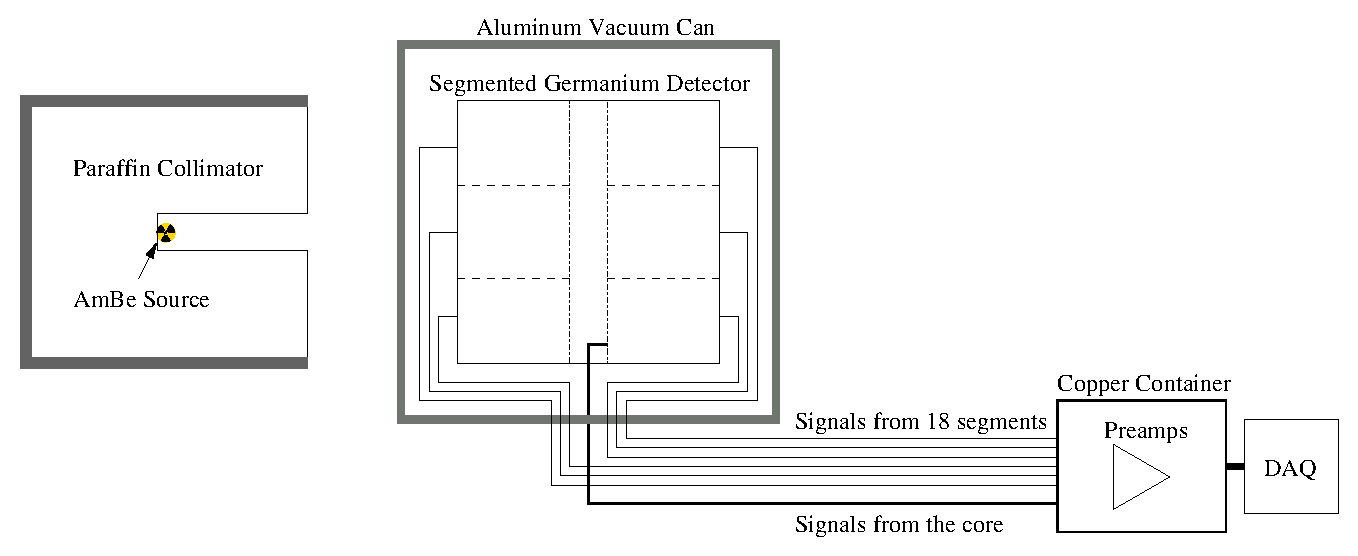
\includegraphics[width=0.95\textwidth]{neuExpSI}
  \caption{Schematic of experimental setup (not to scale).}
  \label{fig:neu:exp}
\end{figure}

The AmBe neutron source had an activity of 1.1~GBq. The energy
spectrum of neutrons emitted from $^{9}$Be$(\alpha,n)^{12}$C$^{*}$
nuclear reaction extends to 12~MeV. High resolution measurements of
such neutron energy spectra are presented in Ref.~\cite{Mar95,
Gei75}. The emittance of photons from the de-excitation of
$^{12}$C$^{*}$ is described in Ref.~\cite{Gei75}.

The front-end electronics and the DAQ system were described in
Sec.~\ref{sec:tt:fend} and Sec.~\ref{sec:tt:daq}, respectively. The
DAQ system was configured such that if two pulses occurred within
240~ns they were added up to a single signal; if the second pulse
occurred 240~ns to 8~$\mu$s after the first one, both of them were
disregarded. Two different gain factors were chosen for four different
measurements. The low gain factor was chosen so that the energy range
up to $\sim 11$~MeV was covered. The high gain factor was chosen for
measurements up to $\sim 3$~MeV. Two measurements were performed with
the AmBe source present. They are referred to as HGdat (High Gain
data) and LGdat (Low Gain data). In order to determine the background
from the laboratory environment two more measurements without the
source were performed. They are referred to as HGbg (High Gain
background) and LGbg (Low Gain background). The data samples with
different gains were combined below 3~MeV. The data sets are listed in
Table~\ref{tab:neu:datset}.

\begin{table}[tbhp]
\centering
\caption{Data sets recorded with and without source.} 
\label{tab:neu:datset}
\begin{tabular}{lcccc}\hline
& \multicolumn{2}{c}{With AmBe Source} & 
\multicolumn{2}{c}{Without AmBe Source} \\\hline
DAQ Gain & High  & Low   & High  & Low  \\
$E_{max}$ [MeV] & $\sim$ 3.5  & $\sim$ 11 & $\sim$ 3.5 & $\sim$ 11 \\
No. of Events & 7.1 M & 4.7 M & 1.5 M & 4.7 M \\
Name & HGdat & LGdat & HGbg & LGbg \\\hline
\end{tabular}
\end{table}

\section{Core spectra}
\label{sec:neu:spec}
The total energy deposited in the germanium crystal was read out
through the core electrode of the detector. Figure~\ref{fig:neu:spec}
shows the core energy spectra for data and background in the range of
[0.08, 3]~MeV. The trigger thresholds were set such that the spectra
above 100~keV were not affected.

\begin{figure}[tbhp]
  \centering
  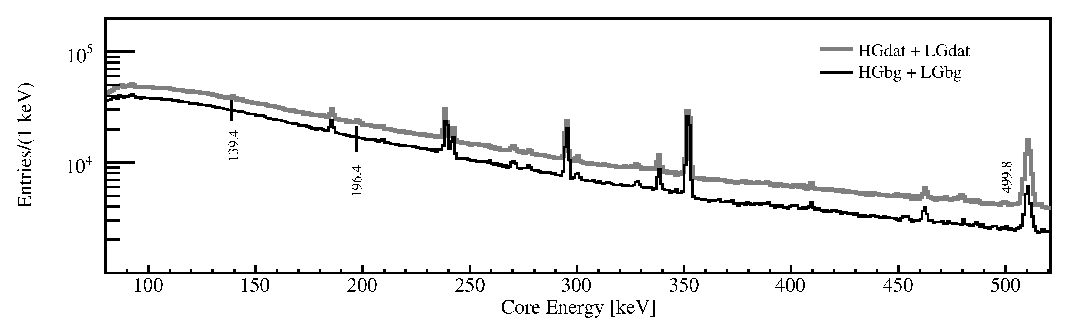
\includegraphics[width=0.9\textwidth,clip]{spectra_0_520keV}
  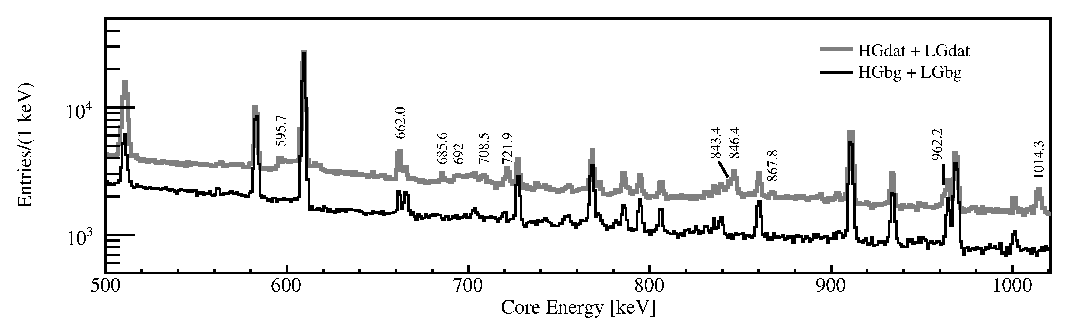
\includegraphics[width=0.9\textwidth,clip]{spectra_500_1020keV}
  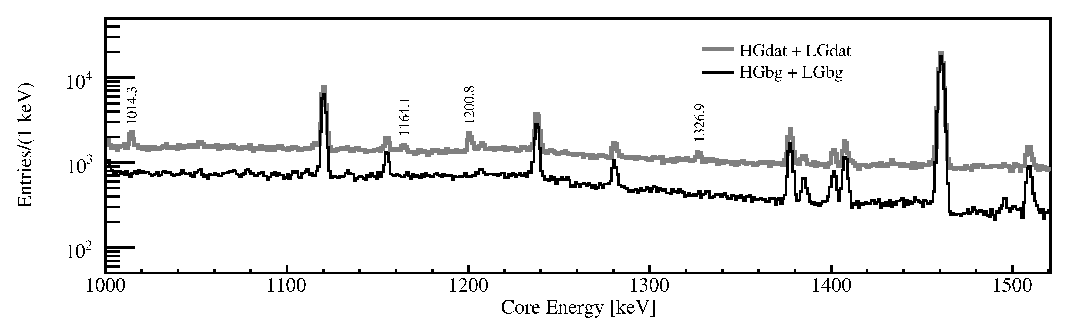
\includegraphics[width=0.9\textwidth,clip]{spectra_1000_1520keV}
  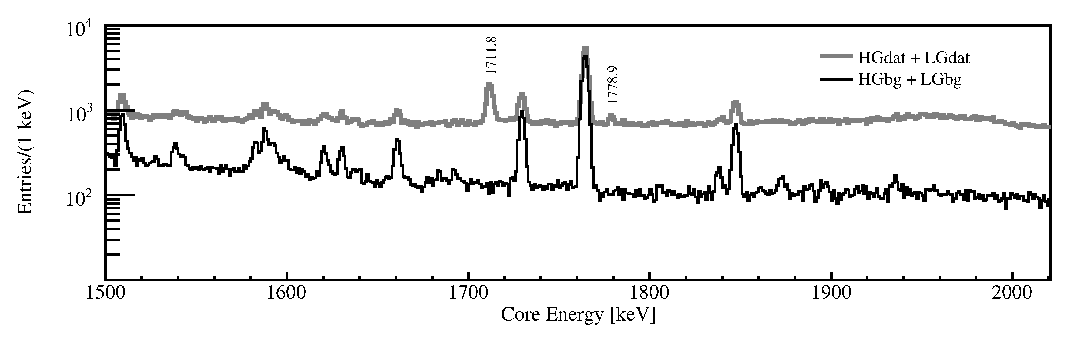
\includegraphics[width=0.9\textwidth,clip]{spectra_1500_2020keV}
  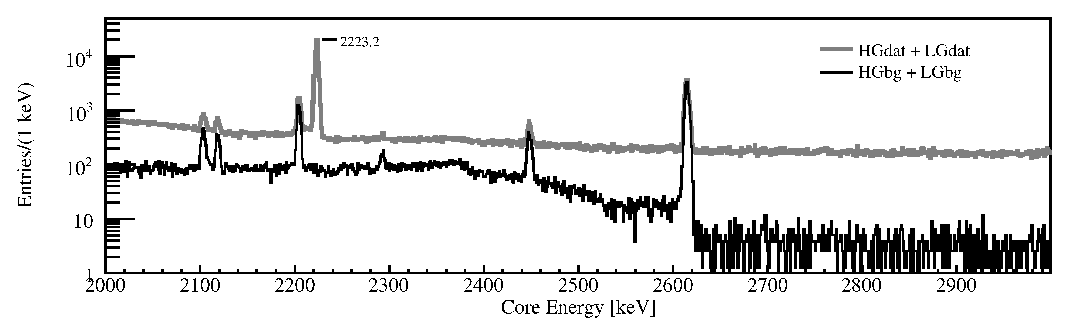
\includegraphics[width=0.9\textwidth,clip]{spectra_2_3MeV}
  \caption{Core energy spectra with and without source. The
    normalization procedure is described in the text. The energy range
    is [0.08, 3]~MeV. Peaks induced by the AmBe source are indicated
    with their energies in keV.}
  \label{fig:neu:spec}
\end{figure}

Figure~\ref{fig:neu:specl} shows the spectra in the range of [3,
10.2]~MeV. In this energy range the background is small, as there are
hardly any radioactive elements producing photons with such high
energies.

\begin{figure}[tbhp]
  \centering
  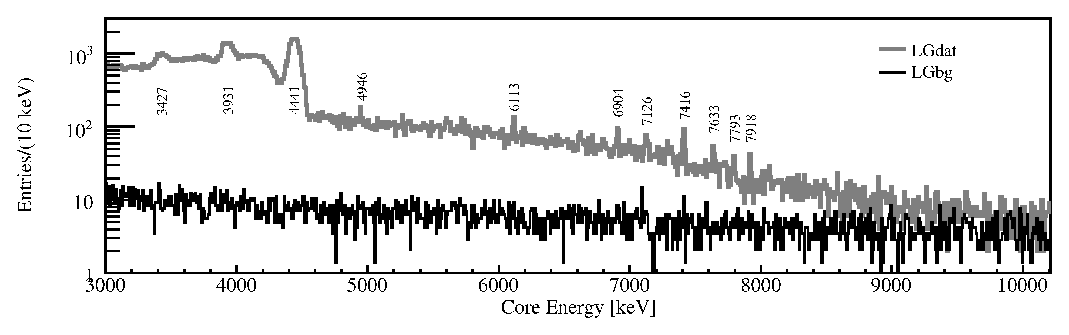
\includegraphics[width=\textwidth,clip]{spectra_3_11MeV}
  \caption{Core energy spectra with and without source. The
    normalization procedure is described in the text. The energy range
    is [3, 10.2]~MeV. Peaks induced by the AmBe source are indicated
    with their energies in keV.}
  \label{fig:neu:specl}
\end{figure}

For Figs.~\ref{fig:neu:spec} and \ref{fig:neu:specl} the background
was normalized using eight photon peaks associated with the decays of
$^{214}$Pb (352~keV), $^{214}$Bi (609~keV, 1120~keV, 1764~keV,
2448~keV), $^{228}$Ac (911~keV), $^{40}$K (1461~keV), and $^{208}$Tl
(2615~keV). A Gaussian function plus a first-order polynomial was
fitted to each peak in data and background. The ratios of numbers of
events in each peak from data and background was taken as scaling
factors. The average, $1.279 \pm 0.003$, was taken as an overall
scaling factor to normalize the background spectrum.

To illustrate the neutron interactions more clearly the normalized
background was subtracted from the data. The resuling spectrum is
shown in Fig.~\ref{fig:neu:specd}. Some of the less prominent
structures were washed out, since a larger bin width was chosen for
statistical reasons.

\begin{figure}[tbhp]
  \centering
  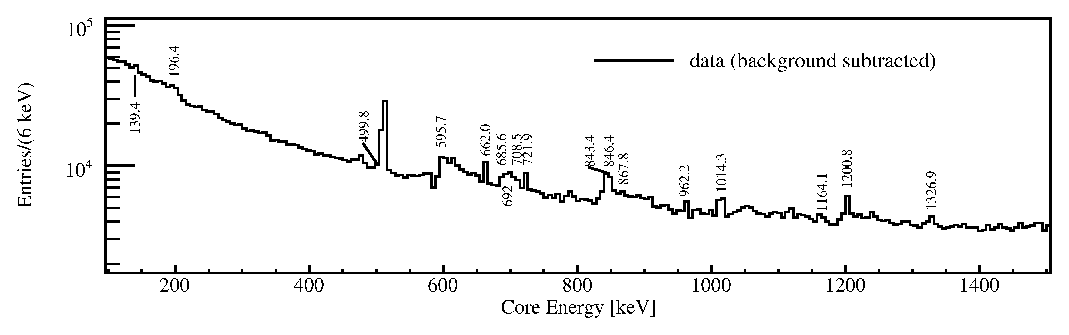
\includegraphics[width=\textwidth,clip]{spectra_0_1d5MeV}
  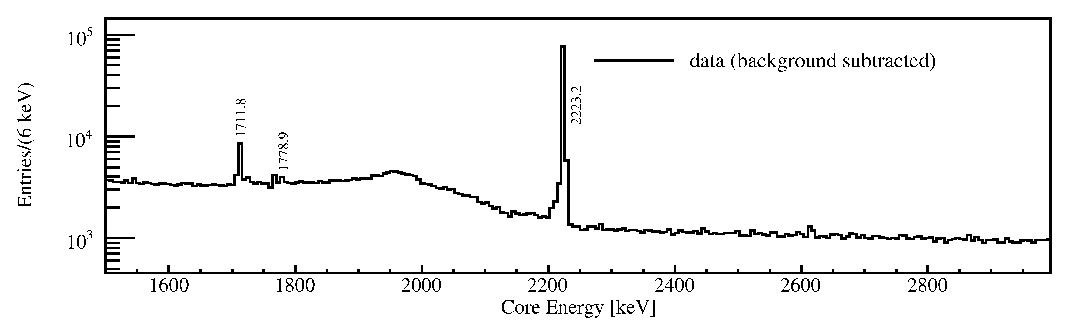
\includegraphics[width=\textwidth,clip]{spectra_1d5_3MeV}
  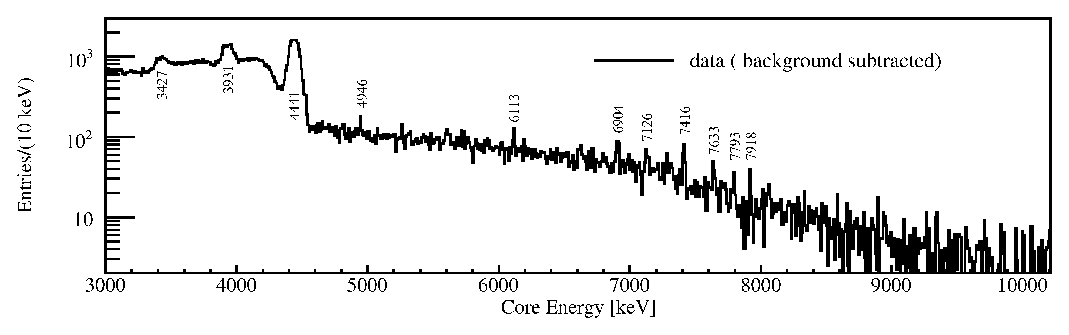
\includegraphics[width=\textwidth,clip]{spectra_3_10d2MeV}
  \caption{Core energy spectra with background subtracted.}
  \label{fig:neu:specd}
\end{figure}

\section{Neutron interactions as seen by the core}
\label{sec:neu:type}
The main interaction mechanisms of neutrons with energies less than
12~MeV are thermal capture, inelastic and elastic scattering. Elastic
scattering does not induce identifiable peaks in the spectrum, because
there is no photon emitted and the recoil energy distribution is too
broad.

The identification of the observed peaks is complex. Not only is the
production mechanism of the excited nucleus important, but the
de-excitation mechanism also has to be taken into account. In most
cases the nucleus de-excites instantaneously with the emission of one
or more photons. However, it can also undergo internal conversion, in
which case an electron from a lower shell is emitted instead of a
photon. The excited nucleus can also be meta-stable and not de-excite
instantaneously.

Table~\ref{tab:neu:type} lists the processes identified in the core
energy spectrum. If inelastic scattering happens inside the germanium
crystal, the nuclear recoil energy is recorded as well as the energies
from some of the prompt photons. In case of instantaneous
de-excitation they are summed up: $E_{inelastic} = E_{\gamma} +
E_{recoil}$. This causes an asymmetric peak with a long recoil tail on
the high energy side. Internal conversions only create identifiable
peaks if they occur inside the crystal, otherwise the emitted
electrons do not reach the detector.

\begin{table}[tbhp]
  \caption{Types of neutron processes identified in the core energy
    spectrum.}
  \label{tab:neu:type}\centering
  \begin{tabular*}{\textwidth}{@{\extracolsep{\fill}}cccc}
    \hline\noalign{\smallskip}
    Production & De-excitation & Symbolic Notation & Short Form \\
    \noalign{\smallskip}\hline\noalign{\smallskip}
    thermal & instantaneous & $n + ^A$Z$ \rightarrow ^{(A+1)}$Z$ +
\gamma$ & $^A$Z$(n,\gamma)$\\
    \noalign{\smallskip}\cline{2-4}\noalign{\smallskip}
    capture & meta-stable 
    & $n + ^A$Z$ \rightarrow ^{(A+1)m}$Z, $^{(A+1)m}$Z$ \rightarrow
^{(A+1)}$Z$+\gamma$ & $^A$Z$(n,\gamma^{m})$\\
    %& & $^{(A+1)m}$Z$ \rightarrow ^{(A+1)}$Z$+\gamma$ & \\
    \noalign{\smallskip}\hline\noalign{\smallskip}
    inelastic & instantaneous & 
    $n + ^A$Z$ \rightarrow ^A$Z$ + n^\prime + \gamma$ &
$^A$Z$(n,n^\prime\gamma)$\\
    \noalign{\smallskip}\cline{2-4}\noalign{\smallskip}
    scattering & internal conversion & 
    $n + ^A$Ge$ \rightarrow ^A$Ge$^{+} + n^\prime + e^-$ &
$^A$Ge$(n,n^\prime e)$\\
    \noalign{\smallskip}\hline
  \end{tabular*}
\end{table}

Table~\ref{tab:neu:peak}, \ref{tab:neu:peak2} list all the peaks
observed in the core energy spectrum due to neutron interactions
within the germanium crystal as well as within the surrounding
materials: H, C, Cl in the paraffin collimator, Al, Ce in the aluminum
vacuum can and Fe, Cu in the support and the detector and electronics
infrastructure.

Purely photon induced peaks were fitted with a Gaussian function plus
a first-order polynomial to get the mean energies, FWHMs and the
numbers of events in the peaks. The 596~keV peak from $^{74}$Ge$(n,
n^\prime \gamma)$ inelastic scattering does not have a Gaussian
distribution. The treatment of this peak is described in
section~\ref{sec:neu:seg}. The 662~keV peak associated with $^{140}$Ce
has a significant background contribution from $^{137}$Cs. This was
subtracted. The 692~keV peak from $^{72}$Ge$(n,n^\prime e)$ is hard to
fit because it is asymmetric and broad. It is also contaminated by
other peaks nearby. The number of events in this peak was estimated by
integration.

The 4.4 MeV peak is due to photons from the de-excitation of
$^{12}$C$^{*}$ created in the AmBe source by the interaction,
$^{9}$Be$(\alpha,n)^{12}$C$^{*}$. It is Doppler broadened because of
the movement of the $^{12}$C$^{*}$ nuclei. The width of this peak
listed in Table~\ref{tab:neu:peak2} was determined by the fit. Because
of low statistics the widths of most of the peaks above 6 MeV had to
be fixed in the fitting procedure according to the detector resolution
around these energies. The peaks that are not identified are marked
with a question mark.

\begin{table}[tbhp]
\centering
\caption{Peaks observed in the core energy spectrum below 3~MeV
(see Fig.~\ref{fig:neu:spec}) due to neutron interactions.} 
\label{tab:neu:peak}
\begin{minipage}{\linewidth}
\begin{tabular*}{\textwidth}{llll} \hline
Fitted Energy~[keV]& Fitted FWHM~[keV]& Interaction Type& Number of Events\\\hline
139.4 & $1.6 \pm 0.2$ & $^{74}$Ge$(n,\gamma^m)$ & $3377 \pm 520$ \\
197.9 & $1.9 \pm 0.2$ & $^{70}$Ge$(n,\gamma^m)$ & $3306 \pm 503$ \\
499.8 & $1.9 \pm 0.7$ & $^{70}$Ge$(n,\gamma)$   & $503  \pm 186$ \\
595.7\footnote{The fitting of the 596~keV peak is described in a later section.} & - & $^{74}$Ge$(n,n^\prime\gamma)$ & $(18.4 \pm 2.5)\times10^3$\\
662.0\footnote{The background contribution to the 662~keV peak was subtracted.} & $1.9 \pm 0.1$ & $^{140}$Ce$(n,\gamma)$ & $2802 \pm 188$ \\
685.6 & $1.4 \pm 0.2$ & ?\footnote{Unidentified peaks are marked with a question mark.} & $628  \pm 111$ \\
692\footnote{The number of events in the 692~keV peak was determined by integration.}  & - & $^{72}$Ge$(n,n^\prime e)$ & $\sim 7000$ \\
708.5  & $2.4 \pm 0.5$ & $^{35}$Cl$(n,\gamma)$,  & $782 \pm 197$ \\
&  & $^{36}$Cl$\rightarrow^{36}$Ar & \\
721.9  & $1.9 \pm 0.2$ & ?$^c$ & $3502 \pm 148$ \\
843.4  & $2.4 \pm 0.5$ & $^{27}$Al$(n,n^\prime\gamma)$ & $1558 \pm 202$ \\
846.6  & $2.4 \pm 0.2$ & $^{56}$Fe$(n,n^\prime\gamma)$ & $2802 \pm 196$ \\
867.8  & $1.9 \pm 0.5$ & $^{73}$Ge$(n,\gamma)$        & $425  \pm 129$ \\
962.2  & $2.4 \pm 0.2$ & $^{63}$Cu$(n,n^\prime\gamma)$ & $1041 \pm 129$ \\
1014.3 & $2.4 \pm 0.2$ & $^{27}$Al$(n,n^\prime\gamma)$ & $1958 \pm 123$ \\
1164.1 & $2.6 \pm 0.5$ & $^{35}$Cl$(n,\gamma)$        & $646  \pm 140$ \\
1200.8 & $2.8 \pm 0.2$ & DEP\footnote{SEP, DEP stand for Single Escape Peak and Double Escape Peak, respectively.} of 2223 & $2318 \pm 122$ \\
1326.9 & $2.4 \pm 0.2$ & $^{63}$Cu$(n,n^\prime\gamma)$   & $711 \pm 91$  \\
1711.8 & $3.8 \pm 0.1$ & SEP$^e$ of 2223 & $5555 \pm 133$ \\
1778.9 & $2.6 \pm 0.2$ & $^{27}$Al$(n,\gamma)$, & $469  \pm 73$ \\
&  & $^{28}$Al$\rightarrow^{28}$Si &  \\
2223.2 & $3.8 \pm 0.1$ & $^{1}$H$(n,\gamma)$    & $79349 \pm 300$ \\
\end{tabular*}
\end{minipage}
\end{table}

\begin{table}[tbhp]
\centering
\caption{Peaks observed in the core energy spectrum above 3~MeV
(see Fig.~\ref{fig:neu:specl}) due to neutron interactions.} 
\label{tab:neu:peak2}
\begin{minipage}{\linewidth}\centering
\begin{tabular*}{\textwidth}{llll} \hline\noalign{\smallskip}
Fitted Energy~[keV]& Fitted FWHM~[keV]& Interaction Type& Number of Events\\\hline
3427 & $85 \pm 7$ & DEP\footnote{SEP, DEP stand for Single Escape Peak and Double Escape Peak, respectively.} of 4441 & $2354 \pm 263$ \\
3931 & $87 \pm 5$  & SEP$^a$ of 4441 & $5873 \pm 368$ \\
4441 & $92 \pm 2$  & $^{9}$Be$(\alpha,n)^{12}$C$^{*}$ & $14672 \pm 297$ \\
4946 & $4.9\pm1.4$ & $^{12}$C$(n,\gamma)$            & $68 \pm 15$     \\
6113 & 7\footnote{The widths were fixed during the fit.} & $^{35}$Cl$(n,\gamma)$ & $75 \pm 12$ \\
6904 & 7$^b$      & SEP$^a$ of 7416            & $60 \pm 10$ \\
7126 & 7$^b$ & ?\footnote{Unidentified peaks are marked with a question mark.} & $38 \pm  9$ \\
7416 & 7$^b$       & $^{35}$Cl$(n,\gamma)$ & $70 \pm 10$ \\
7633 & 7$^b$       & $^{56}$Fe$(n,\gamma)$ & $18 \pm 10$ \\
7793 & $7.1\pm2.1$ & $^{35}$Cl$(n,\gamma)$ & $21 \pm  8$ \\
7918 & $6.8\pm1.4$ & $^{63}$Cu$(n,\gamma)$ & $29 \pm  8$ \\
\end{tabular*}
\end{minipage}
\end{table}

\section{Neutron interactions as seen by the segments}
\label{sec:neu:seg}
The segment energies read out individually provide more information
about the interactions inside the germanium crystal than the core
signal alone.

\subsection{Neutron inelastic scattering}
A special characteristic of neutron inelastic scattering in a
germanium detector is, that not only the photon energy, but also the
recoil energy is recorded. The associated peak in the core spectrum
has a high energy recoil tail and, hence, is much less significant
than a pure photon peak with the same number of events, see
Fig.~\ref{fig:neu:spec}. It is possible to partially separate out the
recoil energy distribution using information from the individual
segments. This is due to the way a segmented detector can provide
information about event topologies.

Figure~\ref{fig:neu:inel} shows the three types of events contributing
to inelastic scattering peaks in the core spectrum. In all cases the
scattered neutron escapes:
\begin{enumerate}
\item the nuclear recoil energy and the prompt photon energy are
deposited in the same segment;
\item the nuclear recoil energy is deposited within one segment, the
prompt photon deposits its energy in several other segments;
\item the nuclear recoil energy is deposited within one segment while
the prompt photon deposits its total energy within another segment.
\end{enumerate}

\begin{figure}[tbhp]
\centering
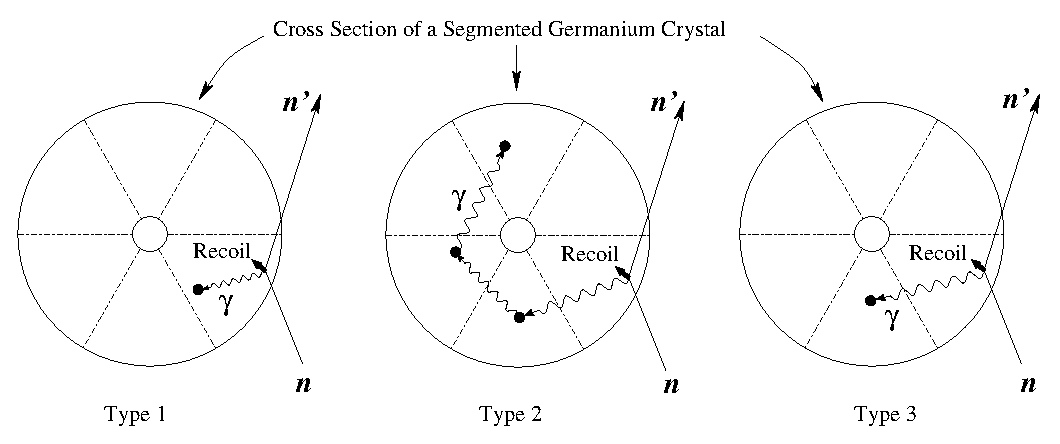
\includegraphics[width=0.8\textwidth]{ine_1}
\caption{Three topologies of neutron inelastic scattering inside a
germanium crystal.}
\label{fig:neu:inel}
\end{figure}

In the first case, only one segment has a signal. The energies
recorded by the core and the segment are the same, i.e. $E_{core} =
E_{seg} = E_{\gamma} + E_{recoil}$. Segmentation cannot help to
disentangle the two energies. In the second case, the recoil energy
can be observed in one segment. As the photon energy is shared between
several segments, there is no peaked distribution in any single
segment. This could partially be recovered by segment energy
summation. In the third case, the recoil energy is observed in one
segment, while the photon is observed in another segment. To
disentangle the photon peak from the recoil energy distribution, 18
energy spectra of all 18 segments are added together\footnote{Each of
the segment provides an energy spectrum. It is the spectra that are
added NOT the energies from the segments.} to get a spectrum of the
energy deposited in \emph{any segment}. In this spectrum, the type~1
events produce the same distribution as in the core spectrum and
type~2 events form a flat distribution. Type~3 events, however, create
a sharp photon peak and an enhancement in the low energy region from
the recoil energy distribution.

Figure \ref{fig:neu:cas} shows the \emph{any segment} spectrum (black)
together with the core spectrum (grey) in the relevant energy
ranges. Three peaks at 596~keV, 834~keV and 1039~keV, associated with
inelastic scattering, $^{74}$Ge$(n, n^\prime\gamma)$, $^{72}$Ge$(n,
n^\prime\gamma)$ and $^{70}$Ge$(n, n^\prime\gamma)$, respectively, are
clearly visible in the \emph{any segment} spectrum. The latter two are
not observable in the core spectrum.

\begin{figure}[tbhp]
\centering
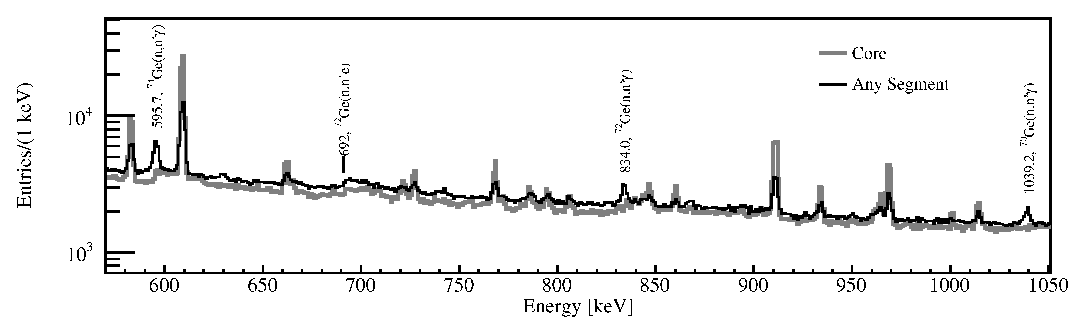
\includegraphics[width=\textwidth,clip]{spe_casp}
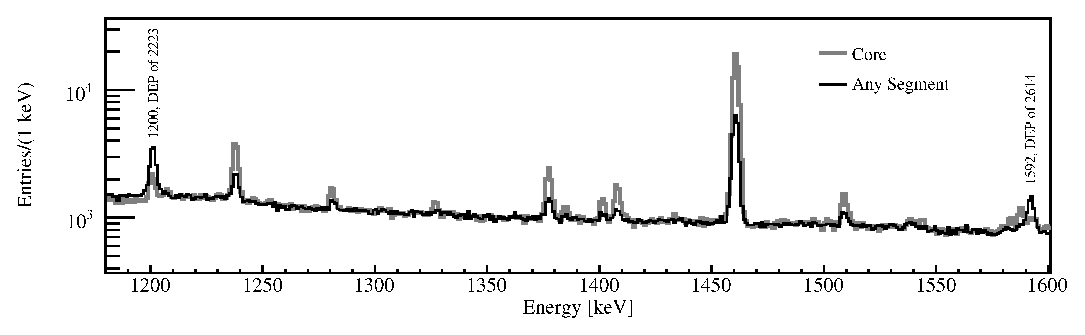
\includegraphics[width=\textwidth,clip]{spe_cas2p}
\caption{The \emph{any segment} spectrum (black) and the core spectrum
(grey) in the relevant energy ranges. The disentangled photon peaks
are much more significant than the original peaks.}
\label{fig:neu:cas}
\end{figure}

It is possible to extract the number of each type of events in the
596~keV peak. The total number of events, $N_{total}$ was determined
from the core spectrum. An exponential function was fitted to the
shoulder of the peak associated with the nuclear recoil energy
distribution. A Gaussian function was fitted to the 609~keV background
photon peak on the shoulder simultaneously. The background below the
recoil structure was obtained from interpolating the spectrum below
and above the shoulder. The total number of events is the difference
between the fitted exponential and the background. The error was
estimated by assuming different levels and shapes of the
background. The fit is shown in Fig.~\ref{fig:neu:f596}.

\begin{SCfigure}[1.4][tbhp]
\centering
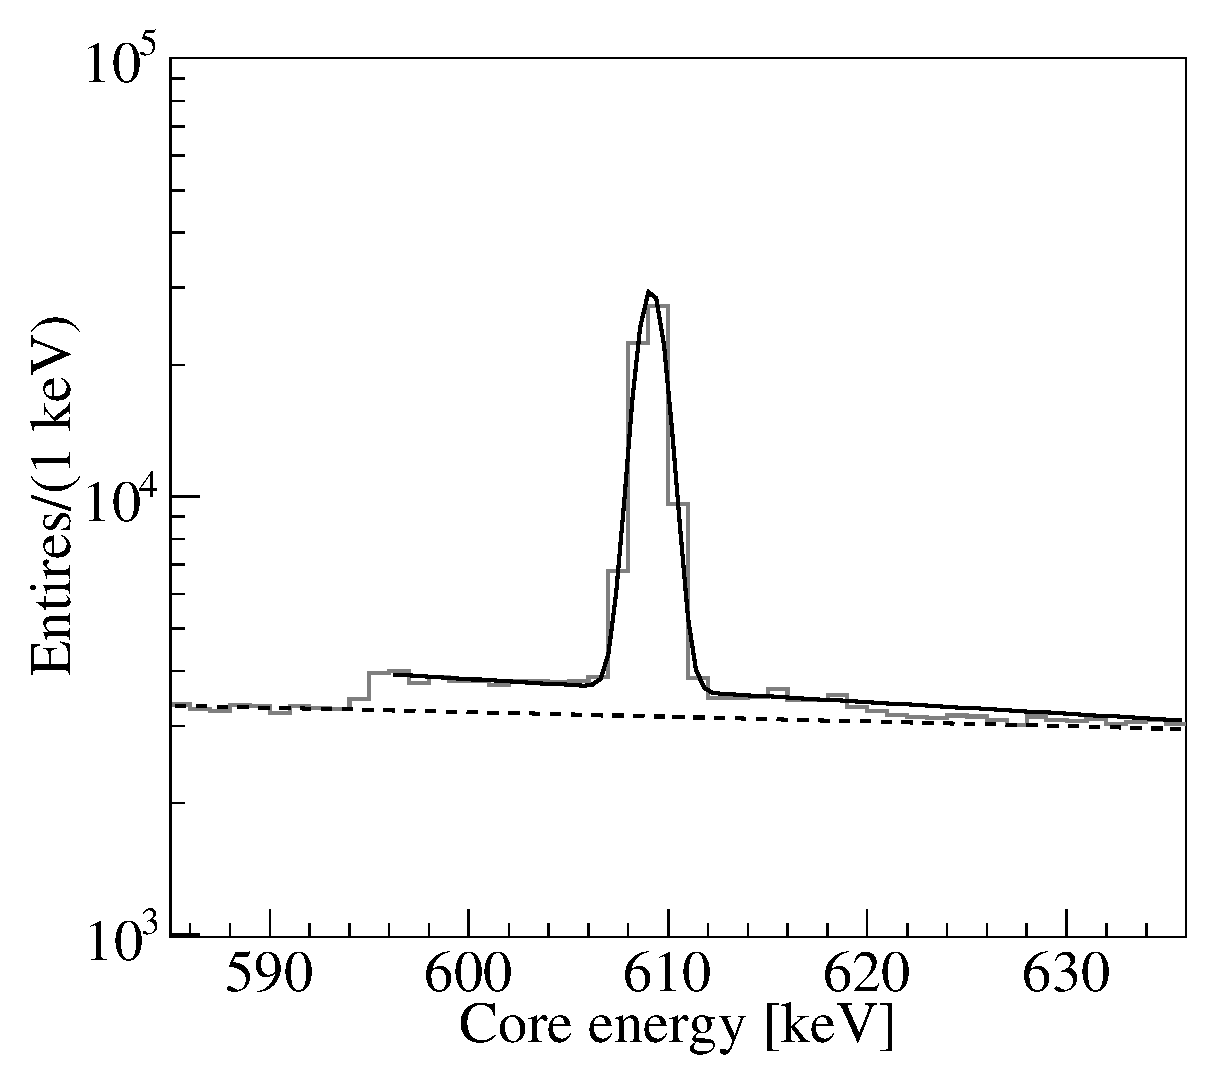
\includegraphics[width=0.4\textwidth]{fit596}
\caption{Close-up of the 596~keV peak in the core spectrum. The dashed
line represents the background, the solid line shows the exponential
plus Gaussian function from the background peak at 609~keV. The
description of the fitting is given in the text.}
\label{fig:neu:f596}
\end{SCfigure}

The number of type~3 events, $N_{type3}$, was obtained by fitting a
Gaussian function plus a first-order polynomial to the 596~keV peak in
the \emph{any segment} spectrum. The small shoulder caused by the
contamination with type~1 events does not change the results of the
fit significantly.

In principle, the number of type~1 events can be determined by fitting
the 596 keV peak in the \emph{single segment} spectrum obtained by
requiring only one segment showing a signal. However, a trigger
threshold of 5~keV had to be used for each segment in order to avoid
electronic noise. Because the recoil energy is often smaller than
5~keV, a lot of type~3 events are recorded as type~1 events. Thus, the
596 keV peak in the \emph{single segment} spectrum contains all the
type~1 events and a large part of type~3 events.

Another way to determine the number of type~1 events requires the
study of the peaks purely induced by photons. This provides the
probability that a de-excitation photon deposits its energy in exactly
one or in multiple segments. The relative strength of the peaks in the
core and any segment spectrum, that is, $\mathcal{R}(E_{\gamma}) =
N_{core}(E_{\gamma}) / N^{any}_{seg}(E_{\gamma}) = (N_{SSE} + N_{MSE})
/ N_{SSE}$, directly translates to the relative rate of the total
number of inelastic scattering events to the sum of type~1 and type~3
events, that is, $\mathcal{R}(E_{\gamma}^{inelastic}) = N_{total} /
(N_{type1} + N_{type3})$.

A Gaussian function plus a first-order polynomial were fitted to
eleven of the most prominent photon induced background peaks in the
core and \emph{any segment} spectra, respectively. The numbers of
events in the peaks from the fits were used to calculate the ratio,
$\mathcal{R}(E_{\gamma})$, see Fig.~\ref{fig:neu:sf}. A second-order
polynomial was fitted to get an estimate of the ratio at any energy,
$\mathcal{R}(E)$. The number of type~1 events can be calculated as
$N_{type1} = N_{total} / \mathcal{R}(E_{\gamma}^{inelastic}) -
N_{type3}$.

\begin{figure}[tbhp]
\centering
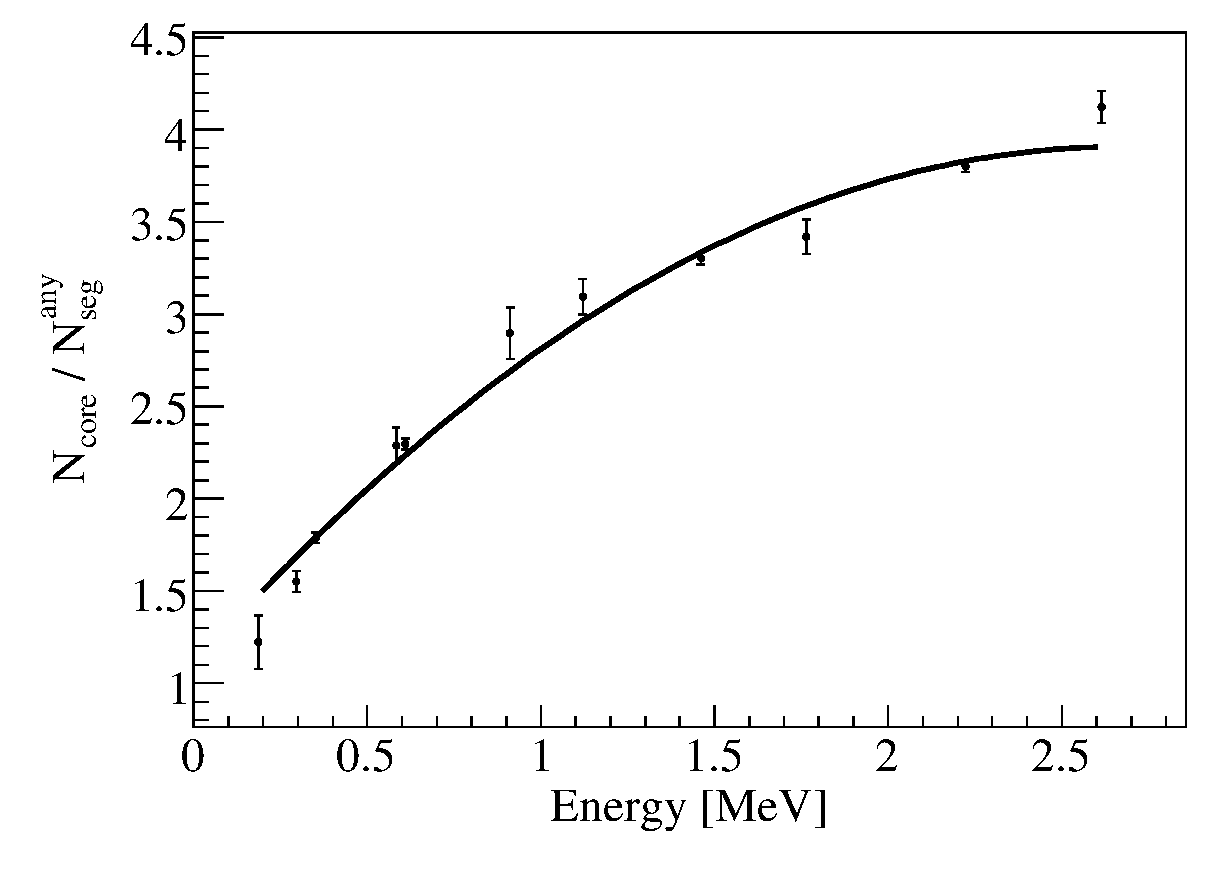
\includegraphics[width=0.6\textwidth,clip]{sf}
\caption{The ``core to any segment ratio'' at the energies of various
photon induced peaks. The errors were taken from the fitting of the
photon peaks. The line is a second-order polynomial fitted to the data
points.}
\label{fig:neu:sf}
\end{figure}

The number of type~2 events can then be calculated as $N_{type2} =
N_{total} - N_{type1} - N_{type3}$. The results concerning event
topologies in the 596~keV peak are listed in the second row of
Table~\ref{tab:neu:ncore}. The percentage of single-segment events,
that is, $N_{type1}$, out of the total number of events is
$\mathcal{P} = N_{type1} / N_{total} \approx 5\%$; \textit{i.e.}, most
events induced by neutron inelastic scattering with the detector are
multi-segment events and can be rejected by requiring only one segment
to show energy.

\begin{table}[tbhp]
\centering
\caption{Numbers of events for different event topologies in the 
596~keV, 834~keV and 1039~keV peaks. Two numbers in square brackets 
indicate the ranges of numbers of events in the 834~keV and 1039~keV 
peaks.}
\label{tab:neu:ncore}
\begin{minipage}{\textwidth}\centering
\begin{tabular*}{\textwidth}{lcccc} \hline\noalign{\smallskip} Energy
[keV] & $N_{type 1}$ & $N_{type 2}$ & $N_{type 3}$ & $N_{total}$ \\
\noalign{\smallskip}\hline\noalign{\smallskip}
595.8 & $1000 \pm 1000$ \footnote{The very large error is due to the propagation of errors of $N_{type3}$, $N_{total}$ and $\mathcal{R}$ according to the relation $N_{type1} = N_{total} / \mathcal{R} - N_{type3}$.} & $(10 \pm 3)\times10^3$ & $7285 \pm 218$ & $(18.4 \pm 2.5)\times10^3$ \\
834.0  & [0, 380] & [4100, 4700] & $2592 \pm 186$ & [6700, 7700] \\
1039.2 & [0, 240] & [2700, 3100] & $1429 \pm 182$ & [4100, 4800] \\
\end{tabular*}
\end{minipage}
\end{table}

The numbers of type~3 events in the 834~keV and 1039~keV peaks were
obtained by fitting the \emph{any segment} spectrum. Since there is no
peak at these two energies in the core spectrum, it is impossible to
get $N_{total}$ from a fit. However, since the percentage $\mathcal{P}
= N_{type1} / N_{total}$ decreases with energy, $\mathcal{P}$ at
834~keV and 1039~keV should be in the range of [0,
$\mathcal{P}$(596~keV)]. Taking into account the relation, $N_{type1}
= N_{total}/\mathcal{R} - N_{type3}$, the ranges of numbers of events
in different topologies in the 834~keV and 1039~keV peaks were
calculated.\footnote{The lower and upper limits in the square brackets
in Table~\ref{tab:neu:ncore} are calculated with $\mathcal{P} = 0$ and
$= \mathcal{P}$(596~keV), respectively} They are listed in
Table~\ref{tab:neu:ncore} as well.

Special events were selected to disentangle the recoil energy,
$E_{recoil}$, spectrum from the photon of energy, $E_\gamma$,
spectrum:
\begin{enumerate}
\item Exactly two segments with an energy deposit above 10~keV were
required.
\item If one segment had an energy deposit in the range
$[E_\gamma-3\sigma, E_\gamma+3\sigma]$, where $\sigma$ was the
detector energy resolution, the energy deposited in the other segment
was used.
\end{enumerate}

The following steps produced the background to the recoil spectra:
\begin{enumerate}
\item Exactly two segments with an energy deposit above 10~keV were
required.
\item Two energy side-bands, $[E_\gamma-6\sigma, E_\gamma-3\sigma]$
and $[E_\gamma+3\sigma, E_\gamma+6\sigma]$ were defined.
\item If one segment had an energy deposit in the side-bands, the
energy deposited in the other segment was used.
\end{enumerate}

Figure~\ref{fig:neu:recoil} shows the disentangled recoil spectra
related to the 596~keV, 834~keV and 1039~keV photon peaks. The
histograms start at 10~keV. Below, the spectra are dominated by
electronic noise. The recoil spectra extending to $\approx 100$~keV
are clearly visible above the background.

\begin{figure}[tbhp]
\centering
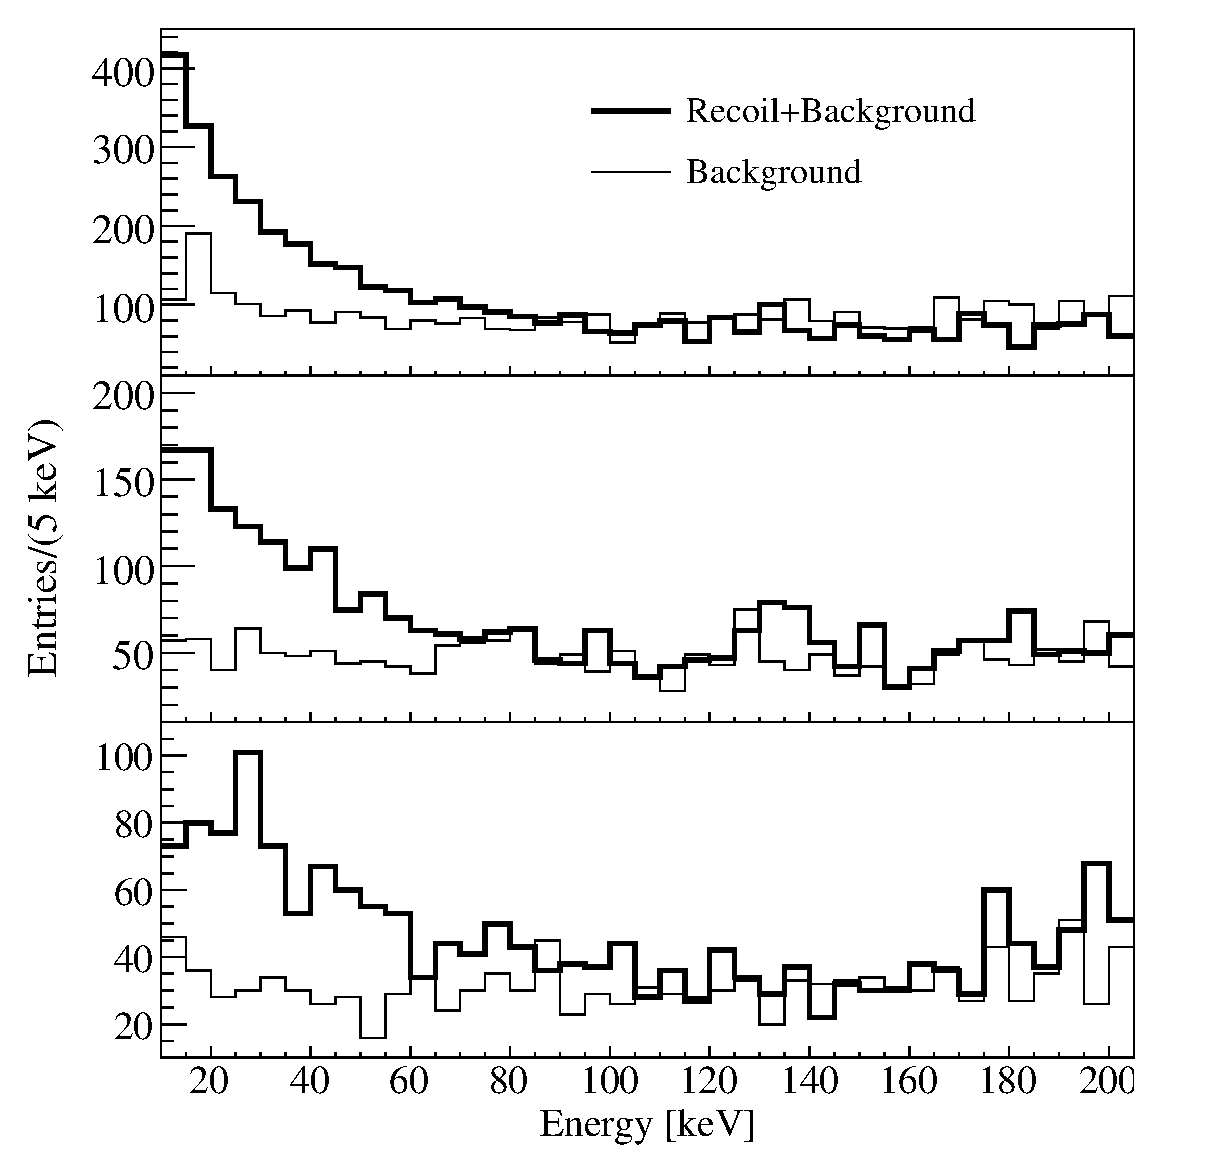
\includegraphics[width=0.6\textwidth]{recoil}
\caption{Measured recoil energy spectra of inelastic neutron
scattering with prompt photons of energies of (a) 596~keV, (b) 834~keV
and (c) 1039~keV.}
\label{fig:neu:recoil}
\end{figure}

\subsection{Internal conversion}
\label{sec:neu:conv}
If the excited state of a nucleus has the same spin as the ground
state, internal conversion \cite{Lis69, Kra56} is the predominant mode
of the de-excitation. Since the mean free path of an electron emitted
from internal conversion is about 1~mm in germanium, the energy of the
electron and the recoil of the nucleus are deposited in the same
segment. The core and the \emph{any segment} spectra are the
same. This is demonstrated in Fig.~\ref{fig:neu:cas}. The 692~keV peak
from internal conversion, $^{72}$Ge$(n,n'e)$, is neither changed nor
suppressed in the \emph{any segment} spectrum.

\subsection{Double escape peaks}
\label{sec:neu:dep}
The photons from neutron induced interactions can subsequently induce
double escape events in pair production. The double escape peaks are
enhanced in the \emph{any segment} spectrum, because many events from
the single escape and full energy peaks in the core spectrum move to
this peak. Two enhanced double escape peaks at 1200~keV and 1592~keV
are clearly visible in Fig.~\ref{fig:neu:cas}. The peak at 1200~keV
originates from the 2223~keV peak of $^{1}$H$(n,\gamma)$ thermal
capture. The 1592~keV peak originates from the 2614~keV peak of
$^{208}$Tl; This is not a neutron induced interaction.


\section{Verification of simulation}
\label{sec:neu:sim}
The Geant4 \cite{Gea03, Gea06} based simulation package MaGe, as
described in Sec.~\ref{sec:ph:sim}, was used to simulate the
experiment. The version Geant4 8.2 with patch-01 was used.

\subsection{Generator, geometry and physics processes}
\label{sec:simdetail}
The neutron spectrum of an AmBe source taken from Fig.~5 in
Ref.~\cite{Mar95} was normalized to a probability density function and
used in the neutron generator to assign energies to the outgoing
neutrons. The generator also produced 4.4 MeV photons from the
$^{12}$C$^{*}$ de-excitation inside the AmBe source. The Doppler
broadening of the 4.4 MeV peak was simulated by Gaussian smearing with
the observed widths taken from Table~\ref{tab:neu:peak2}.

The geometry of the experiment was implemented according to the
technical drawings. Approximations up to several centimeters had to be
made regarding
\begin{itemize}
\item the shape and size of the AmBe source and how it was held inside
the paraffin collimator,
\item the exact relative positions of the crystal and the paraffin
collimator,
\item the exact geometry of the components inside the cryostat.
\end{itemize}

Geant4 provides high precision models for the simulation of
interactions of neutrons with energies below 20~MeV \cite{Gea03,
Gea06}. The models rely on the ``evaluated neutron data library''
(G4NDL) for cross sections, angular distributions and final state
information. The version G4NDL3.10 was used.

\subsection{Core spectrum}
\label{sec:neu:spemc}
Figure~\ref{fig:neu:mca} shows the simulated core energy spectrum. The
threshold effects below 100~keV were not taken into account in the
simulation. Figure~\ref{fig:neu:mc} compares the simulation with the
measurement in the range of [0.1, 3]~MeV. The background was
normalized to data as described in section \ref{sec:neu:spec}. The
simulation was normalized to data according to the relation, $N_{data}
= N_{background} + N_{signal} = N_{background} + N_{simulation}$,
where the $N$s are the event numbers in the data, background and
simulated spectra. Figure~\ref{fig:neu:mcl} shows the same spectra in
the range of [3, 10.2]~MeV.

\begin{figure}[tbhp]
  \centering
  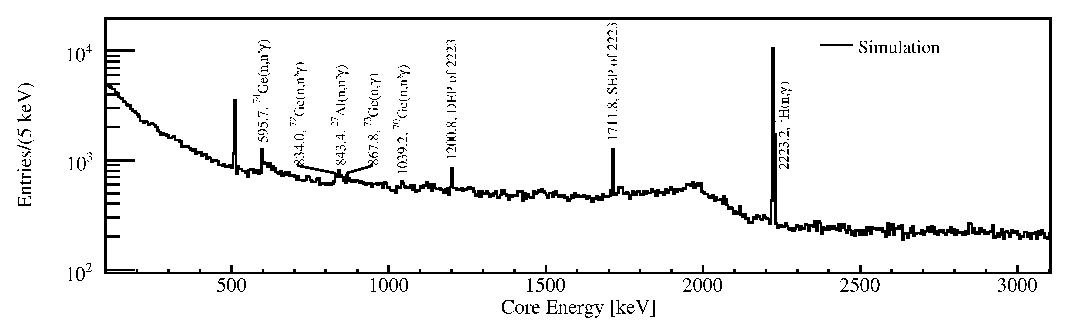
\includegraphics[width=\textwidth,clip]{spectra_mc1}
  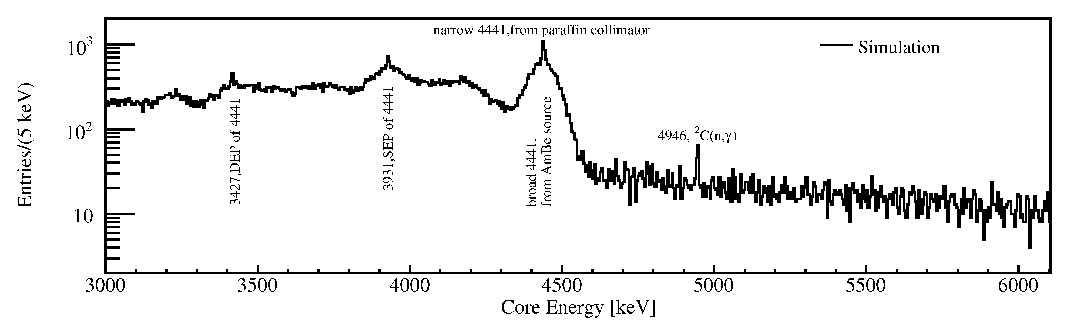
\includegraphics[width=\textwidth,clip]{spectra_mc2}
  \caption{Simulated core energy spectrum from 0.1~MeV to 6.1~MeV.}
  \label{fig:neu:mca}
\end{figure}

\begin{figure}[tbhp]
  \centering
  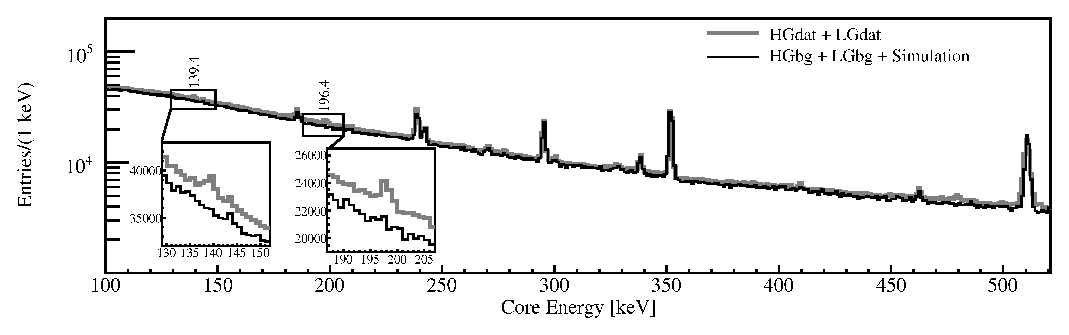
\includegraphics[width=0.9\textwidth,clip]{spectra_0_520keVm}
  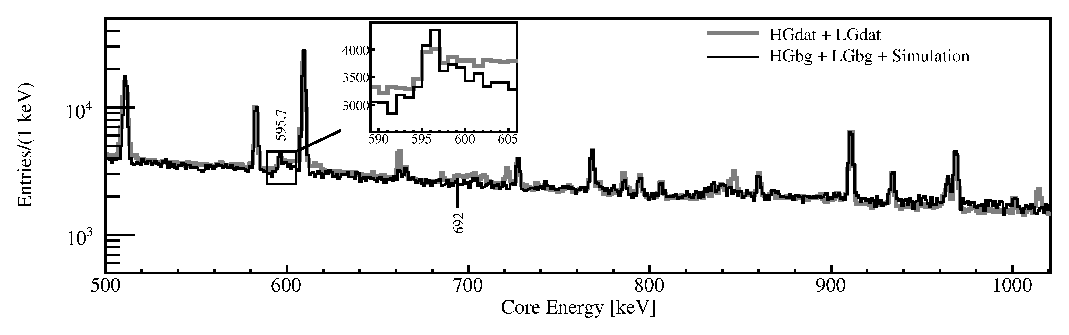
\includegraphics[width=0.9\textwidth,clip]{spectra_500_1020keVm}
  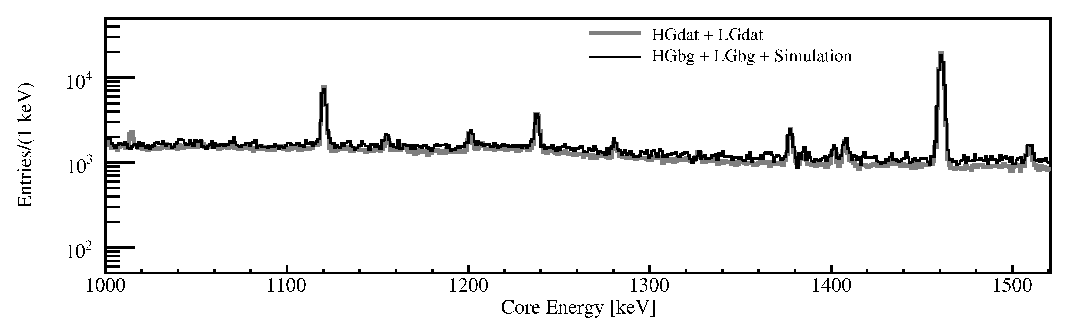
\includegraphics[width=0.9\textwidth,clip]{spectra_1000_1520keVm}
  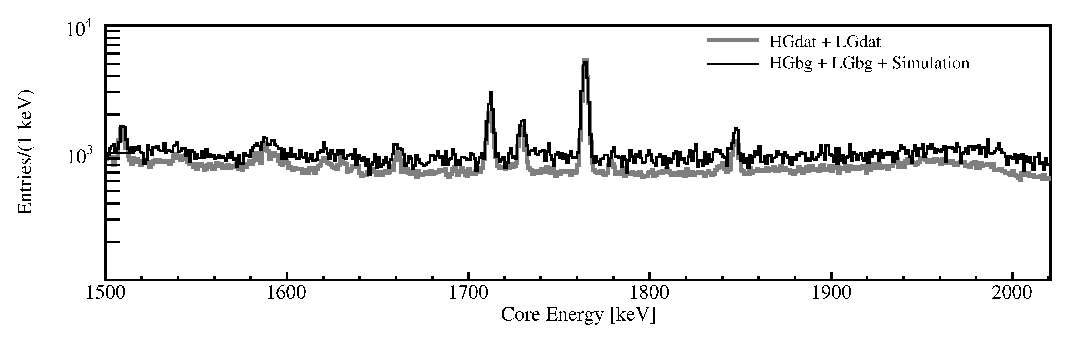
\includegraphics[width=0.9\textwidth,clip]{spectra_1500_2020keVm}
  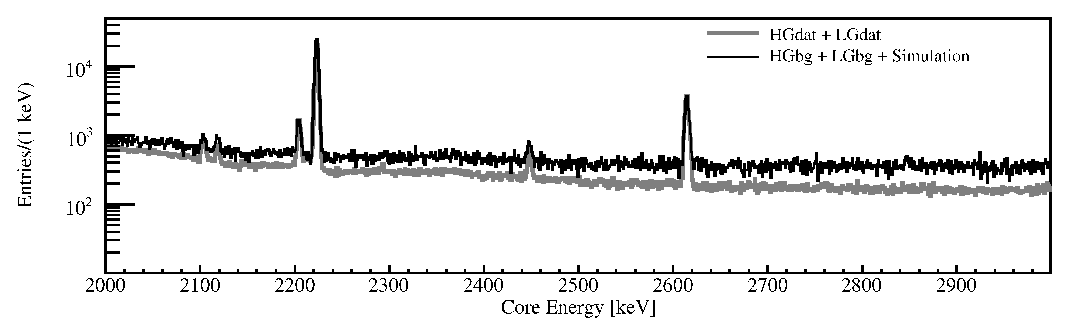
\includegraphics[width=0.9\textwidth,clip]{spectra_2_3MeVm}
  \caption{Comparison of the neutron core energy spectrum from 0.1~MeV
    to 3~MeV between data and simulation plus measured background.}
  \label{fig:neu:mc}
\end{figure}

\begin{figure}[tbhp]
  \centering
  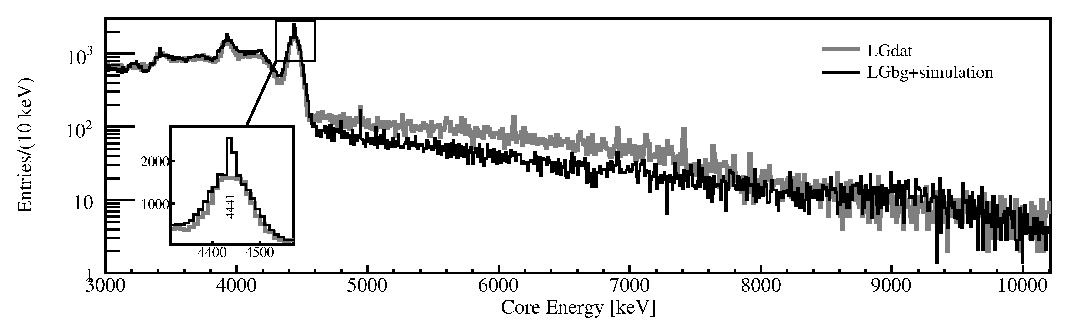
\includegraphics[width=\textwidth,clip]{spectra_3_11MeVm}
  \caption{Comparison of the neutron core energy spectrum from 3~MeV to
    10.2~MeV between data and simulation plus measured background.}
  \label{fig:neu:mcl}
\end{figure}

\subsection{Discrepancies between data and simulation}
\label{sec:neu:dine}
In general the simulation describes the data very well. Some
discrepancies are discussed here.

The shapes of the continuous spectra from the simulation and data
above $\approx 1.5$~MeV deviate due to the poor knowledge of the exact
material and geometry of components between the source and the
crystal.

There is a known bug \cite{g4bug1} in Geant4 concerning neutron
inelastic scatterings. The secondary particles are not boosted back to
the laboratory frame after the calculations in the center of mass
frame are completed. This causes two problems:
\begin{itemize}
\item The simulated recoil energies of the germanium nuclei are wrong.
\item The photon peaks from these interactions are not broadened.
\end{itemize}

The first effect is demonstrated in the third inset of
Fig.~\ref{fig:neu:mc}. The measured 596~keV peak from
$^{74}$Ge$(n,n^\prime\gamma)$ has a long tail on the high energy side
due to the nuclear recoil while the simulated peak misses this
feature.

The second effect is demonstrated by the inset of
Fig.~\ref{fig:neu:mcl}.  The simulation generates a broad and a narrow
peak, both at 4.4~MeV.  The broad peak is due to the de-excitation of
$^{12}$C$^{*}$ created in the source. The generator was adjusted to
describe the data. The narrow one is due to neutron inelastic
scattering on carbon atoms in the paraffin collimator,
$^{12}$C$(n,n'\gamma)$. In reality, the carbon atom can gain a
velocity of up to $0.02c$ causing a Doppler broadening of the order of
50~keV-100~keV. This is comparable to the broadening in the
$^{12}$C$^{*}$ de-excitation peak, and can, thus, not be resolved in
the measured spectrum.

Another problem was observed in connection with the
$^{1}$H$(n,\gamma)$ photon peak of 2223~keV. The mean value from a
Gaussian fit to this peak is $(2223.24 \pm 0.01)$~keV. The simulated
peak centers at $(2224.61 \pm 0.01)$~keV. This shifted value comes
from the evaluated neutron data library. The problem was reported to
the Geant4 Problem Tracking System \cite{g4bug2}. It was fixed for our
studies by correcting the value in the database. The result is shown
in Fig.~\ref{fig:neu:h2223}.

\begin{figure}[tbhp]
\centering
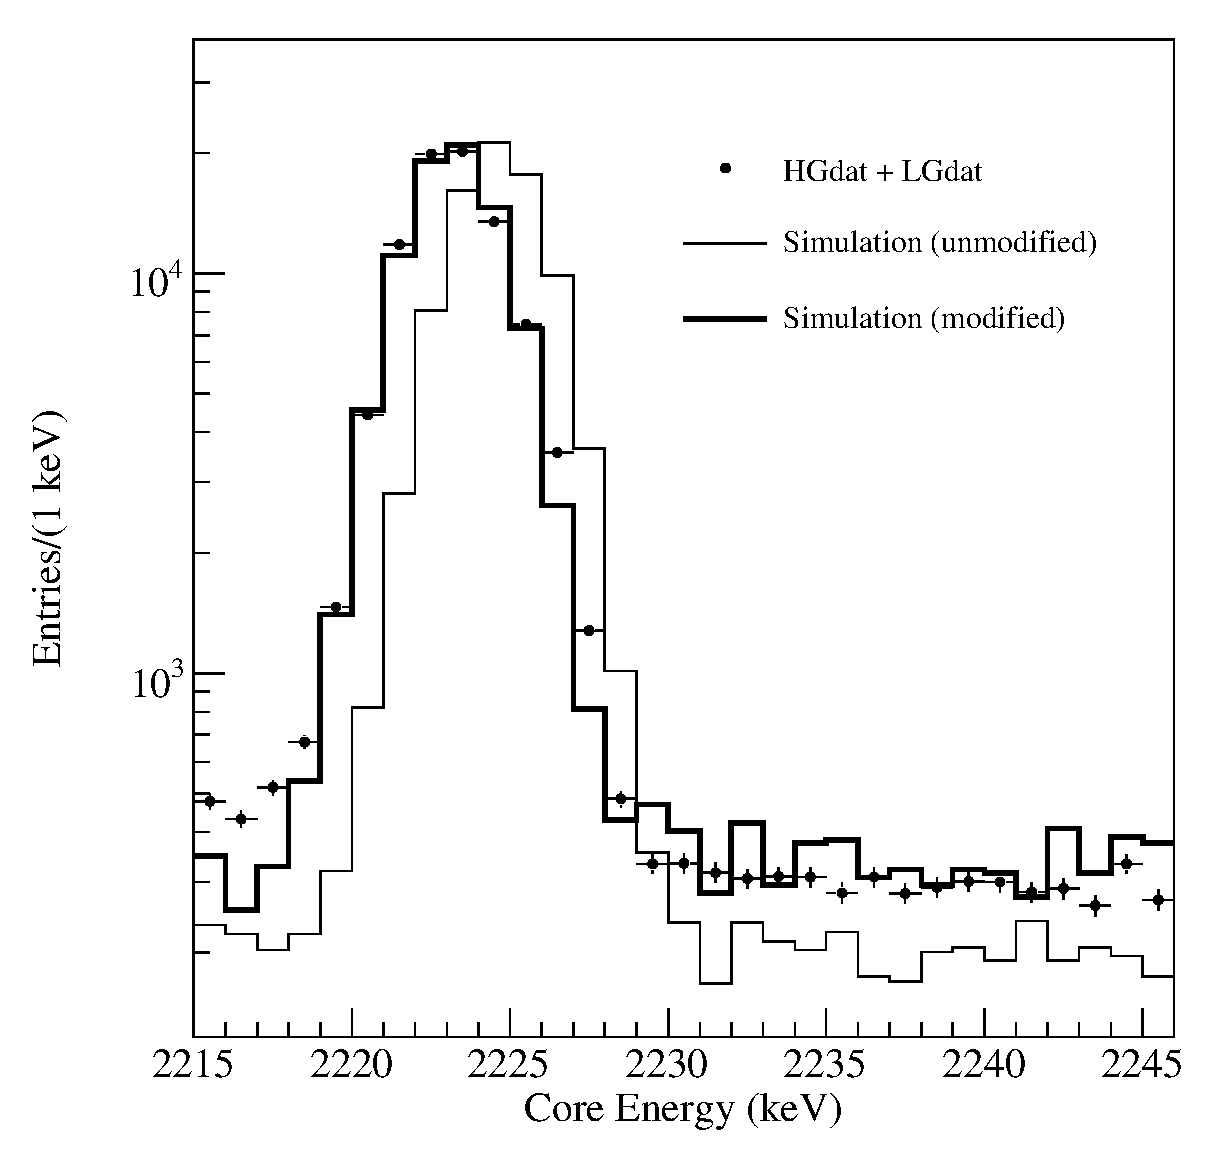
\includegraphics[width=0.6\textwidth]{h2223}
\caption{The 2223~keV photon peak from $^{1}$H$(n,\gamma)$ in data and
simulation. The spectra were normalized according to the numbers in
the photon peaks. The simulated peak was shifted to 2224.6~keV before
the modification described in the text.}
\label{fig:neu:h2223}
\end{figure}

The 139~keV and 196~keV photon peaks from the meta-stable states of
$^{75}$Ge and $^{71}$Ge produced by neutron capture are missing in the
simulated neutron spectrum, see the first two insets of
Fig.~\ref{fig:neu:mc}. This problem has been reported to the Geant4
Problem Tracking System \cite{g4bug3}.

The 692~keV peak from internal conversion, $^{72}$Ge$(n,n^{\prime}e)$,
is also missing in the simulation, see Fig.~\ref{fig:neu:mc}. Again,
this was reported \cite{g4bug4}.

\section{Summary}
\label{sec:neu:out}
The 18-fold segmented germanium detector, Siegfried I, was exposed to
an AmBe neutron source and spectra were taken. A number of peaks from
neutron interactions on germanium isotopes as well as the surrounding
materials were identified. It was proven that neutron inelastic
scattering mainly produces multi-segment events which can be rejected
by requiring only one segment showing energy. The segment information
was proven to be very helpful in identifying peaks induced by neutron
inelastic scattering, hence can be used to improve our understanding
of the background for GERDA.

The Geant4 based simulation package, MaGe, was used to simulate the
experiment. While the description was in general very good, several
discrepancies between data and MC were found. Most of them were
corrected. Some further verification and improvement of the related
Geant4 codes are needed.


%%% Local Variables:
%%% mode:latex
%%% TeX-master: "thesis"
%%% End:
